\documentclass[a4paper,two column]{article}
    \usepackage[utf8]{inputenc}
    \usepackage[english]{babel}
    \usepackage{amsmath}
    \usepackage{amssymb}
    \usepackage{amsthm}
    \usepackage{graphicx}
    \usepackage{hyperref}
    \usepackage[top=1in, bottom=1.25in, left=1in, right=1in]{geometry}
    \usepackage{wrapfig}
    % \theoremstyle{definition}
    % \newtheorem{definition}{Definition}[section]
    % \theoremstyle{remark}
    % \newtheorem*{remark}{Remark}
    % \newtheorem*{theorem}{Theorem}
    \usepackage[autostyle]{csquotes}
    \usepackage{float}
    \usepackage[font={small,it}]{caption}
    \usepackage[title]{appendix}
    \usepackage{subfig}
    \usepackage[export]{adjustbox}
    \title{Understanding Tunneling in many body system with a toy model}
    \author{Biplab Mahato\thanks{$3^{rd}$ year Undergraduate, Indian Institue of Science, \href{mailto:biplab@iisc.ac.in}{biplab@iisc.ac.in}}}
    \begin{document}
    \maketitle
        \tableofcontents
        \section{Introduction}\label{sec:Introduction}
            Understanding Quantum Tunneling of an entity having its own internal degrees of freedoms through a potential barrier is a fundamental problem in physics as well as in chemistry. Nuclear fusion is one such area where study of quantum tunneling in many body system become essential \ref{ref:nuclearfusion}. Many formalisms like Coupled Channel formalisms, are proposed to understand this phenomenon. This report rather take a simplistic approach to the problem. Report starts with the statement of the problem followed by a baby model to understand it and finally to conclude, results are presented from multiple calculations using the baby-model.
        \section{The Problem}\label{sec:problem}
            Consider a scattering experiment with two nuclei. It can be either both of them approaching each other(in the lab frame), or one is in rest while the other in motion. As they scatter off each other many interesting thing can happen because of their internal structure. Nucleus are not like rigid balls so as they "collide" (come close to each other while scattering) their will certainly be deformities in their structures. More interestingly the nuclei after scattering might be different altogether then the nuclei to start with. One possibilty is that they  can exchange an alpha particle. This exchange of alpha particle happens through quantum tunneling through the high potential barrier (which was responsible for the formation of the surface of nucleus before scattering). Now this tunneling can happen in both direction (in fact tunneling probabilties for tunneling to either side of the potential is equal irrespective of the shape of the potential (it might not be symmetric)). So if an alpha particle somehow tunnel through the potential barrier to the other nucleus then after some time if nuclei are kept as it is alpha particle will come back to its parent nucleus. This time interval can be called the reccurance time. So if an experiment is set up which allows the nuclei to interact for long enough (way larger than the reccurance time) then possibility (cross-section) of such alpha particle transfer will be less. While if the experiment is carried out fast enough (interaction time smaller than recurrance time possibly half of it) then such process will be physically realisable with very high success rate. So the goal of this report is to estimate the reccurance time.  
        \section{The Formalism}\label{sec:formalism}
            \subsection{Potential}\label{subsec:potential}
                Exact form of potential energy due to nucleus is not known. Empherical equations of various form has been proposed(see \ref{ref:nuclearpotential}). For example potential energy due to two nucleons are approximated by Reid potential\ref{ref:reid}(shown in the figure\ref{fig:reidpotential}). Note several feature of the potential. Far apart nucleons does not impart any significant effect on each other due to short rangeness of strong force. At small distance force is attractive while even smaller distance it become highly repulsive. Now we need to know the potential which originate from two nuclei at a distance and an alpha particle travelling to and forth. In principle it is hard to guess the time dependent potential. But in this toy model we will assume the potential to look like a symmetric double well potential. For two similar heavy nuclei this is a reasonable choice as it captures the essence that two nuclei are the potential wells and to go to and forth alpha particle has to tunnel through the barrier in the middle. Though for this toy model details of the potential is not needed.
                \begin{figure}[H]
                    \centering
                    \subfloat[Reid Potential]{{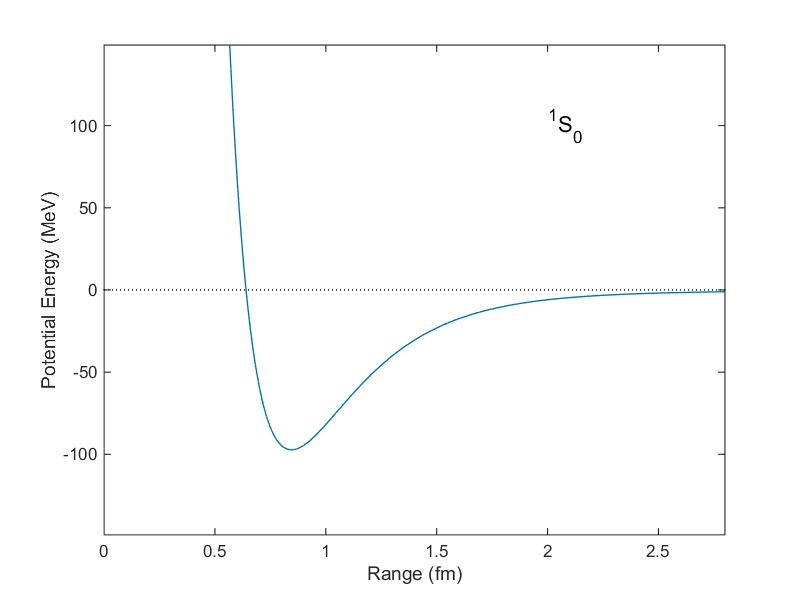
\includegraphics[width=0.435\textwidth,fbox]{image/ReidPotential.jpg}}}
                    \qquad
                    \subfloat[Symmetric Double well potential]{{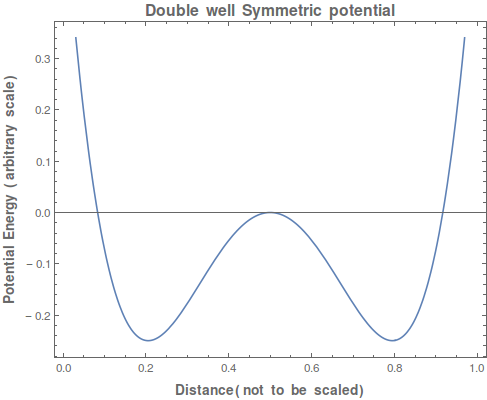
\includegraphics[width=0.4\textwidth,fbox]{image/doublewell}}}
                    \caption{Potentials: a)potential due to two nucleons b) Double well potential}
                    \label{fig:reidpotential}
                \end{figure}
            \subsection{The Over-simplified Model}\label{subsec:oversimplifiedmodel}
                A symmetric potential have all its stationary wave functions as either symmetric or antisymmetric (they alternate in energy). Two well potential also admits such stationary states lowest being a symmetric one(for a single particle in it). Lowest two levels looks something like the figure below. \\
                We will label those states as $|+\rangle$ and $|-\rangle$. For the simplicity of the model we will pretend that the well has only these two levels and nothing else. So $|+\rangle$ and $|-\rangle$ form the basis of the Hilbert space of the system corresponding to this potential. Though more intutive basis will be 
                \begin{eqnarray}
                    |L\rangle = \frac{1}{\sqrt{2}}(|+\rangle+|-\rangle)\\
                    |R\rangle = \frac{1}{\sqrt{2}}(|+\rangle-|-\rangle)
                \end{eqnarray}
                where  $|L\rangle$ and  $|R\rangle$ respectively correspond to the states where the particle is solely confined to the left and right of the potential barrier. \\
                As $|+\rangle$ and $|-\rangle$ are the eigenstates of the Hamiltonian and they form the basis any state can be written as $|\Psi\rangle = a|+\rangle + b|-\rangle $ and its time evolution will be 
                \begin{equation}
                    |\Psi(t)\rangle = a |+\rangle + b e^{-i\epsilon t}|-\rangle
                \end{equation}
                where $\epsilon$ is the energy gap between $|+\rangle$ and $|-\rangle$ and $\hbar$ is taken to be 1. This also implies that probability of coming back to the same state 
                \begin{equation}
                    |\langle\Psi(0)|\Psi(t)\rangle|^2 = | |a|^2 + |b|^2 e^{-i\epsilon t}|^2 
                \end{equation}
                it is easy to see that after time $T = 2\pi / \epsilon$ any state comes back to the original state. So recurrance time for this system is $ 2\pi / \epsilon$.
            \subsection{Simplified Model}\label{subsec:simplifiedmodel}
                The above model does capture the bare minimum essence of the problem but one can do better. The alpha particle also have internal structures which will affect the system for example it so happen that after tunneling into the right well alpha particle may be disintegrated (absorbed into the nucleus). These phenomenon can be incorporated into the above system just by introducing internal states of the alpha particle. Note the Hibert space of internal states can be combined with the Hilbert space of the earlier system just by taking tensor product. Also we can introduce coupling by introducing various off-diagonal term in the Hamiltonian.
                So for a system of two potential having two states and the particle having two (simplified) internal states (separated by an energy gap $\delta$) Hamiltonian will look in the basis left right and two internal stationary states $\left\{|L0\rangle,|L1\rangle,|R0\rangle,|R1\rangle\right\}$.
                \begin{equation}
                    H  = \begin{pmatrix}
                        \epsilon/2&0&-\epsilon/2&0\\
                        0&\epsilon/2 + \delta &0&-\epsilon/2 + \delta\\
                        -\epsilon/2&0&\epsilon/2&0\\
                        0&-\epsilon/2 + \delta &0&\epsilon/2 + \delta\\
                    \end{pmatrix}
                \end{equation}
                One can also introduce the coupling as follows.
                \begin{equation}\label{Hamiltonian}
                    H = \begin{pmatrix}
                        \epsilon/2&0&-\epsilon/2&0\\
                        0&\epsilon/2 + \delta &0&-\epsilon/2 + \delta\\
                        -\epsilon/2&0&\epsilon/2&V\\
                        0&-\epsilon/2 + \delta &V&\epsilon/2 + \delta\\
                    \end{pmatrix}
                \end{equation}
                where it is assumed that whenever particle is in the right side of the well it gets coupled with the excited internal state. 
            \subsection{Solution of the toy model}\label{subsec:solutiontoymodel}
                Now that we set up our Hamiltonian we can in principle solve the system. Also as this is only a $4$by$4$ Hamiltonian, numerical techniques can also be used without much computational effort. Though there is a clever way to find the recurrance time. Is eigenvalues and eigenvectors of the Hamiltonian (\ref{Hamiltonian}) are $\{E_i,v_i\}$ then any state can be written as a linear combination of the $v_i$'s. $|\Phi\rangle = \sum_{i=1}^{4} c_i |v_i\rangle$. And the state will evolve as 
                \begin{equation}
                    |\Phi(t)\rangle = \sum_{i=1}^{4} c_i e^{-iE_i t} |v_i\rangle
                \end{equation}
                Each of the term $c_i  e^{-iE_i t}$ comes back to the original value after $T_i = 2\pi/E_i$. So the whole state will come back to initial state after $T = lcm(T_i)$ time. Here definition of lcm has to be reviewed since $T_i$'s will be real number whereas lcm only applies to the integers. So we have to turncate the reals upto certain decimal and then multiply it with suitable no to get an integer and then only taking lcm will make sense(multiplied number also has to devided at last). 
            
        \section{Results and Discussions}\label{sec:results}
            For all the calculations below particle is assumed to be starting from the state $|L0\rangle$ unless mentioned otherwise. Toy model is best understood by changing its parameters($\epsilon,\delta $ and $V$) one by one.\\
            \begin{itemize}
            \item \underline{\textbf{$\mathbf{\delta = V = 0}$:}} Without $\delta$ and V the model reduce to the basic model in section \ref{subsec:oversimplifiedmodel}. Then $a=b=\frac{1}{\sqrt{2}}$ and so 
            $|\langle L |\Psi(t)\rangle|^2 = \frac{1}{4}|1 + e^{-i\epsilon t}|^2 = cos^2(\frac{\epsilon t}{2})$. So  the recurrance time is $\frac{2\pi}{\epsilon}$. 
            \begin{figure}[H]
                \centering
                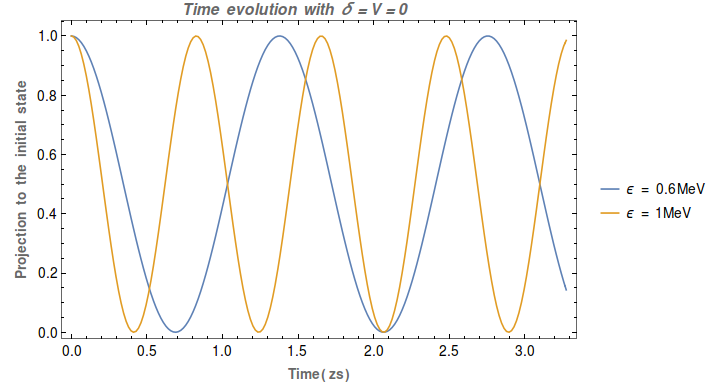
\includegraphics[width=0.45\textwidth,fbox]{image/twowell_epsilon1del0V0}
                \caption{Projection to the initial state varies sinusoidally if $\delta = V = 0$; Increasing $\epsilon$ increases the frequency of oscilation.}
                \label{fig:epsilonoscillation}
            \end{figure}
            \item \underline{\textbf{$\delta=0,V$ small:}} Introduction of a small coupling parameter will create an oscillation between $|0\rangle$ and $|1\rangle$. But as we have seen time period of this oscillation goes like $\frac{1}{energy}$, one would expect low frequency oscillation due to V compared with $\epsilon$. So when both $\epsilon$ and small V is present in the model an envelope due to V oscillation can be seen over the normal $\epsilon$ oscillation.
            \begin{figure}[H]
                \centering
                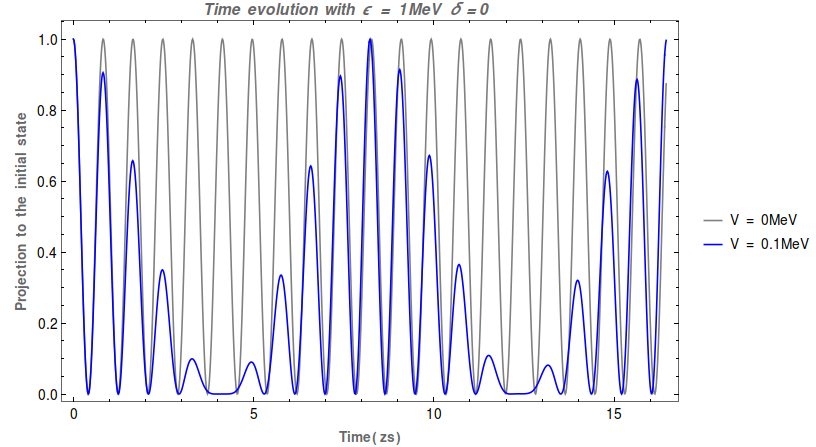
\includegraphics[width=0.45\textwidth,fbox]{image/twowell_epsilon1del0V}
                \caption{Oscillation of the projection to the initial state with small V; Oscillation without V is shown in the background.}
                \label{fig:smallV}
            \end{figure}
            \item \underline{\textbf{$\delta=0,V $ large:}} Following the argument in the last paragraph, for large V oscillation due to only V will be too fast( higher frequency) compared to the $\epsilon$ oscillation. So the particle which went to the right well and thrown into the excited internal state comes back to the ground state very quickly and so $\epsilon$ oscillation doesnot change much but just get modulated by the V oscillation.
            \begin{figure}[H]
                \centering
                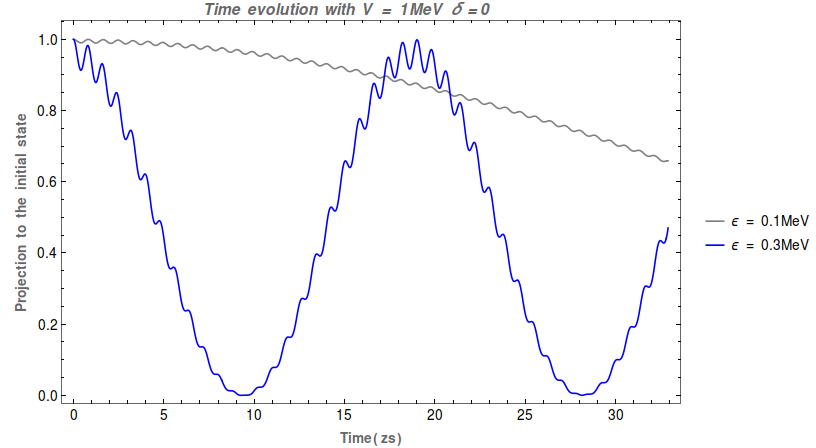
\includegraphics[width=0.45\textwidth,fbox]{image/twowell_epsilondel0V1}
                \caption{Oscillation with large V; Oscillation at different $\epsilon$ is shown}
                \label{fig:largeV}
            \end{figure}
            \item \underline{\textbf{$All non-zero$:}} Introduction of non-zero $\delta$ in the model somehow increases the projection on the initial state. The projection never goes to zero which means all the states orthogonal to $|L0\rangle$ are not attained in the time evolution. 
            \begin{figure}[H]
                \centering
                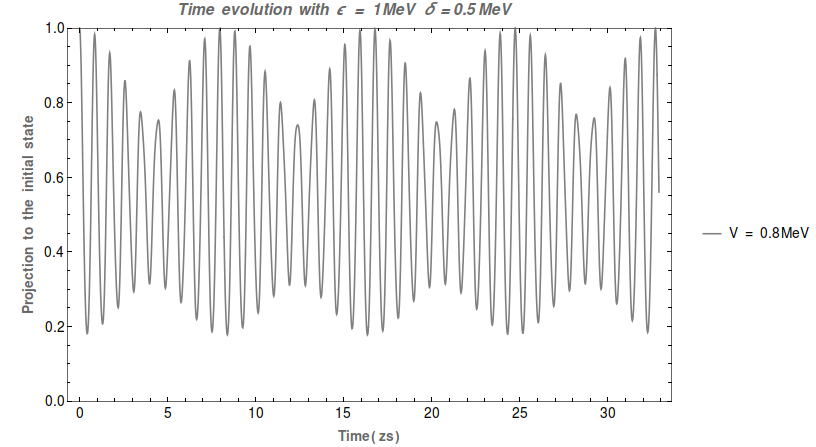
\includegraphics[width=0.45\textwidth,fbox]{image/twowell_epsilondelV}
                \caption{Oscillation in presence of both $\delta$ and V in the model.}
                \label{fig:allnonzero}
            \end{figure} 
            \item \underline{\textbf{LCM method:}} As described in the subsection \ref{subsec:solutiontoymodel}, one can just diagonalise the Hamiltonian and take the lcm of $\frac{2 \pi}{E_i}$. A python code is used to implement this which gives following results.
            For fixed $\epsilon=1MeV$ and $\delta = 0.8MeV$ time period changes with V as follows
            \begin{figure}[H]
                \centering
                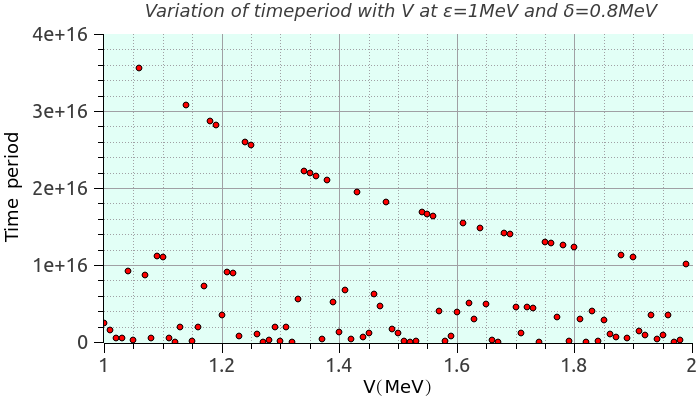
\includegraphics[width=0.45\textwidth,fbox]{image/variationV}
                \caption{LCM of the inverse of the eigenvalues. Strong order can be seen for higher values of time periods while lower values seem random.}
                \label{fig:variationV}
            \end{figure}
            There is no apparent pattern apart from  a "cut-off" curve for large time periods. Primary suspect for this kind of behaviour is the instability of the code. The code tries to find the lcm of a few rational numbers (in principle irrational number also) after turncating at certain decimal point(By multipling $10^n$). If the ingeers after turncating become even then naturally lcm decreases hence the time period. So we expect sudden decrease in time period (by a factor of 2 or sometime even more) which featured in the above plot. Now if we only consider the orderly higher values of time period and plot the logarithm of it to fit against a linear graph we obtain folloing fit which gives $T \approx V^{-1.38}$.
            \begin{figure}[H]
                \centering
                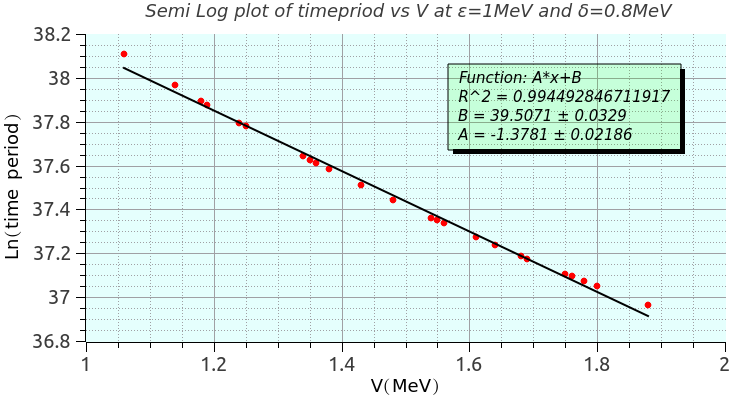
\includegraphics[width=0.45\textwidth,fbox]{image/semilogvariationV}
                \caption{Linear fit of the semi-log plot of only the orderly higher values of time periods.}
                \label{fig:semilogplot}
            \end{figure} 
            \end{itemize}
        \section{Future Directions}
            This model can be improved significantly for example one can introduce more internal states and see how that effect the results. Also time-dependent Hamiltonian can be used as one expect changes in the energies as nucleus approach each other. As an example a time dependent Hamiltonian where epsilon changes linearly from 0 to 2 MeV and then comes back to 0 MeV gives following projection
            \begin{figure}[H]
                \centering
                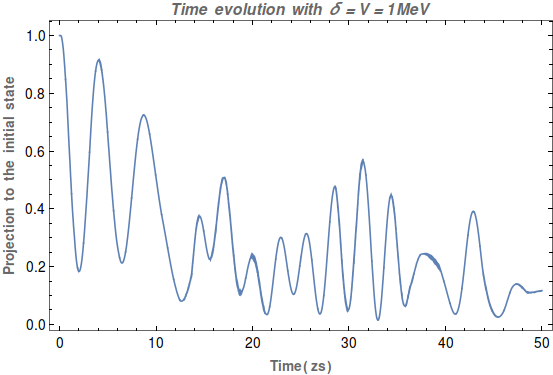
\includegraphics[width=0.45\textwidth,fbox]{image/changeepsilonlin2v1d1}
                \caption{Projection to the initial state as $\epsilon$ changes linearly from 0 to 2MeV and then back to 0MeV.}
                \label{fig:timedependentlin}
            \end{figure}
        \section{References}\label{References}
            \begin{enumerate}
                \item A. B. Balantekin, N. Takigawa 1998. Quantum tunneling in nuclear fusion. Rev. Mod. Phys. 70, 77 \label{ref:nuclearfusion}
                \item Roderick V Reid Jr. 1968. Local phenomenological nucleon-nucleon potentials. Annals of Physics
                Volume 50, Issue 3, Pages 411-448 \label{ref:reid}
                \item Naghdi, M. (2014) Comparing some nucleon-nucleon potentials. Phys. Part. Nuclei Lett. Volume 11, Issue 4, pp 410–431 \label{ref:nuclearpotential}
            \end{enumerate}
    \end{document}